% select subfiles base file
\documentclass[TGAI_Laborbericht.tex]{subfiles}
\begin{document}


\chapter{Versuch 1}
\label{chap:VERSUCH_1}


\section{Fragestellung, Messprinzip, Aufbau, Messmittel}
\label{chap:VERSUCH_1_FRAGESTELLUNG}

\subsection*{Fragestellung}
Es soll die Kennlinie eines Abstandssensores ermittelt werden. Dazu sollen wir 20 Messungen im Abstand von 10 bis 70cm mithilfe eines Oszilloskopes per Hand, als auch per USB an den PC im Labor übertragen. Anschließend sollen die Mittelwerte ermittelt werden, um ein genaues Messergebnis zu gewährleisten. Hinzu kommt noch die Berechnung der Standartabweichung. Das ganze soll dann noch Grafisch dargestellt werden.

\subsection*{Messmittel}
Als Messmittel dienten ein Oszilloskop als Messgerät, sowie ein Entfernungsmesser als
Sensor. Das Oszilloskop ist das Modell TDS 2022B des Herstellers Tektronix und ist via USB mit einem PC im Labor verbunden. Der Entfernungssensor war ein Distanzsensor vom Typ GP2Y0A21YK0F der
Firma Sharp, welcher nach dem Triangulationsprinzip funktioniert.

\subsection*{Aufbau}
Der Aufbau erfolgte, indem das Oszilloskop sowie der Sensor miteinander verbunden wurden und beide Geräte an ein Netzgerät mit 5V Gleichspannung angeschlossen wurden.
Danach gab es noch eine Einweisung in das Oszilloskop. Gegenüber vom Sensor wurde eine kleine Holzspanplatte als zu messendes Objekt platziert. Diese Holzplatte wurde im Abstand von 13-70cm dann in gleichmäßigen abständen von je 3cm nach hinten verrückt, um verschiedene Messergebnisse zu erhalten.

\subsection*{Messprinzip}
\begin{flushleft}
Das Messprinzip des Abstandsensoren beruht auf Zwei Linsen. Hinter der ersten Linse sitzt eine Infrarot-LED und hinter der zweiten Linse sitzt ein optischer Positionssensor (OPS, engl. position sensitive detector PSD). Die LED sendet nun einen schmalen Lichtstrahl aus, welcher von Objekten welche vor dem Sensor liegen reflektiert wird. Je nachdem wie nun der reflektierte Strahl in den OPS fällt wird dessen Leitfähigkeit beeinflusst. Die Leitfähigkeit wird nun mithilfe eines Signalprozessors in eine Spannung umgewandelt welche an den Ausgang des Sensors abgegeben wird.
\begin{figure}
	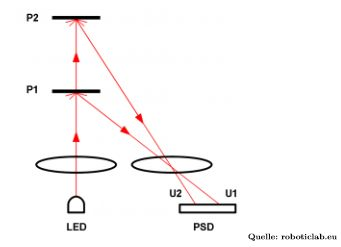
\includegraphics[width=0.7\textwidth]{media/Sharp.jpg}
	\caption{Sensorprinzip}
	\label{fig:Sensor}
\end{figure}
\par
Der Sensor hat die Eigenschaft, dass sein Ausgangssignal anti-proportional ist. Anti-proportional heißt, dass sich das Ausgangssignal mit größerer Entfernung verringert. Zusätzlich ist die Maximale Messdistanz durch zwei Dinge beschränkt:
\begin{itemize}
\item Die Menge des reflektierten Lichtes nimmt mit der Entfernung ab.
\item Das Auflösungsvermögen des OPS ist begrenzt. Weit entfernte Objekte können so nicht mehr unterschieden werden.
\end{itemize}
Hinzu kommt noch, dass der Sensor einen Mindestabstand hat, der je nach Baureihe zwischen 4-20 cm variiert. Das kommt daher, weil der Output steil abfällt sobald eine bestimmte Entfernung unterschritten wird. Der empfohlene Messbereich beträgt 10-80cm.
\par

\end{flushleft}

\section{Messwerte}
\label{chap:VERSUCH_1_MESSWERTE}
\begin{flushleft}
Wie oben beschrieben, wurden 21 Messversuche im Abstand von je 3 cm sowie die
Seitenlängen und Breite eines DinA4 Blattes ermittelt. Diese Ergebnisse wurden vom
Oszilloskop abgelesen und per Hand in ein Blatt eingetragen, diese Messwerte können Sie
folgender Tabelle entnehmen:
\begin{table}[H]
\begin{tabular}{|c|c|c|}
Entfernung & Spannung & V \\ 
\hline 
10 cm & 1,34 V & 56,0 mV \\ 
\hline 
13 cm & 1,23 V & 56,0 mV \\ 
\hline 
16cm & 1,06 V & 56,0 mV \\ 
\hline 
19cm & 0,93 V & 56,0 mV \\
\hline 
22cm & 0,87 V & 56,0 mV \\
\hline 
22cm & 0,87 V & 56,0 mV \\
\hline 
25cm & 0,80 V & 56,0 mV \\ 
\hline 
28cm & 0,752 V & 56,0 mV \\
\hline
31cm & 0,704 V & 56,0 mV \\
\hline
34cm & 0,664 V & 56,0 mV \\
\hline
37cm & 0,632 V & 56,0 mV \\
\hline
40cm & 0,600 V & 56,0 mV \\
\hline
43cm & 0,608 V & 56,0 mV \\
\hline
46cm & 0,544 V & 56,0 mV \\
\hline
49cm & 0,520 V & 56,0 mV \\
\hline
52cm & 0,488 V & 56,0 mV \\
\hline
55cm & 0,440 V & 56,0 mV \\
\hline
58cm & 0,432 V & 56,0 mV \\
\hline
61cm & 0,408 V & 56,0 mV \\
\hline
64cm & 0,328 V & 56,0 mV \\
\hline
67cm & 0,384 V & 56,0 mV \\
\hline
70cm & 0,360 V & 56,0 mV \\
\hline
\end{tabular}
\label{Messwerte per Hand}
\caption{Messwerte per Hand} 
\end{table}
	

	
	



Anzumerken sei noch, dass wir zum Teil durch einen Ablesefehler falsche werte in die Tabelle eingetragen haben.
Neben dem ablesen per Hand, wurden die Messwerte noch per USB verbindung an den PC im Labor übertragen und mithilfe der Software "OpenChoice Dekstop" ausgelesen und im "csv\dq ~Excel format gespeichert. 
\end{flushleft}

\section{Auswertung}
\label{chap:VERSUCH_1_AUSWERTUNG}
\begin{flushleft}
Zur auswertung und verarbeitung der Messwerte, verwenden wir die Bibliothek "Numpy" welche wir in der Skriptsprache Python verwenden. Der erste Schritt zur auswertung der Daten, besteht darin die Dateien mit den Messwerten einzulesen. Dies erfolgt mithilfe des Numpy befehls "genfromtxt", welcher uns aus einer Textdatei ein Array von Daten erstellt. Da wir die Dateien nach dem Schema z.B 13cm.csv abgespeichert haben, können wir dies ganz einfach mithilfe einer Schleife bewerkstelligen. Beim Einlesen der Daten ist noch zu beachten, dass wir erst in der Zeile 1000 mit dem Einlesen beginnen. Dies wird in der Versuchsanleitung empfohlen, da sich der Sensor erst einpendeln muss. 

Nun berechnet man für jede Messung den Mittelwert. Dies erfolgt mit der Numpy funktion "mean". Hier werden alle Werte addiert und durch die Anzahl der Messwerte dividiert.
\begin{figure}[H]
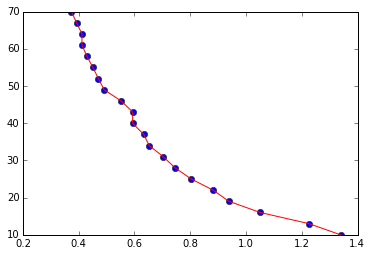
\includegraphics[]{media/messwerte.png}
\caption{Mittelwerte}
\end{figure}
Als nächstes brauchen wir noch die jeweilige Standartabweichung. Für diese brauchen wir die Funktion \dq std\dq ~ ebenfalls aus der Numpy Bibliothek.
\end{flushleft}

\section{Interpretation}
\label{chap:VERSUCH_1_INTERPRETATION}
Man kann erkennen, dass sich die Mittelwerte wie eine Exponentialfunktion verhalten. Genauso erhöt sich die Standartabweichung mit zunehmender Distanz vom Sensor.
\end{document}